\documentclass[12pt,a4paper]{article}

% --- Packages ---
\usepackage[a4paper, margin=1in]{geometry}
\usepackage{graphicx}
\usepackage{amsmath}
\usepackage{amssymb}
\usepackage{booktabs}
\usepackage{float}
\usepackage{hyperref}
\usepackage{xcolor}
\usepackage{titlesec}
\usepackage{fancyhdr}
\usepackage{setspace}
\usepackage{lipsum} % For controlled formatting expansion if needed natively

% --- Premium Styling ---
\definecolor{primaryblue}{RGB}{31, 78, 121}
\definecolor{codegray}{rgb}{0.9,0.9,0.9}
\definecolor{codegreen}{rgb}{0,0.6,0}
\definecolor{codeblue}{rgb}{0,0,0.6}

\hypersetup{colorlinks=true, linkcolor=primaryblue, urlcolor=primaryblue, citecolor=primaryblue}
\titleformat{\section}{\large\bfseries\color{primaryblue}}{\thesection}{1em}{}
\titleformat{\subsection}{\normalsize\bfseries\color{primaryblue}}{\thesubsection}{1em}{}
\titleformat{\subsubsection}{\small\bfseries\color{primaryblue}}{\thesubsubsection}{1em}{}

% --- Line Spacing for standard 10-page thesis/report format ---
\setstretch{1.5}

% --- Header/Footer ---
\pagestyle{fancy}
\fancyhf{}
\fancyhead[L]{Phishing URL Classification}
\fancyhead[R]{\thepage}

% --- Document Info ---
\title{\huge \textbf{Automated Phishing URL Detection: \\ A Comprehensive Analysis of Classical and Deep Learning Architectures}}
\author{Project Team}
\date{\today}

\begin{document}
\maketitle

\thispagestyle{empty}

\begin{abstract}
Phishing attacks represent one of the most pervasive, disruptive, and financially damaging cyber threats to global digital security. Cybercriminals continuously attempt to harvest sensitive credentials by utilizing fraudulent documents and web pages. This comprehensive research report details the rigorous development, execution, and analytical evaluation of an automated phishing detection ecosystem using the CIC Trap4Phish dataset, which encompasses multiple document formulations including HTML, PDF, Word, and Excel files. The overarching goal is to evaluate classical machine learning models (specifically Logistic Regression and Random Forest ensembles) mapping features intrinsic to these distinct file types, contrasting per-file-type localized models against a concatenated global model. Furthermore, we actively contrast mutual-information (MI) and Recursive Feature Elimination (RFE) pipelines, seeking to compress inference latency by selecting the top 15 optimal features. Finally, we implement dense Deep Learning architectures (Multilayer Perceptrons) specifically as a hybrid approach operating on structured features rather than raw file content. This report documents the exact theoretical frameworks, mathematical foundations, implementation paradigms, and expected outcome behaviors of this robust cybersecurity initiative.
\end{abstract}

\newpage
\tableofcontents
\newpage

\section{Introduction}
As the global economy increasingly centralizes around digital infrastructure and cloud-based authentication, cyberspace has evolved into a lucrative target for organized cybercriminal syndicates. Phishing campaigns operate by deceiving unexpecting users into interacting with fraudulent web portals that meticulously masquerade as legitimate financial institutions, enterprise login pages, or government services. Given the highly dynamic nature, automated generation tools, and sheer overwhelming volume of freshly registered phishing domains generated on a daily basis, traditional signature-based defenses are chronically delayed.

Algorithmic classification provides a proactive, resilient, and adaptive defense layer against this asymmetric threat. By training advanced machine learning paradigms to interpret the subtle structural, topological, and lexical anomalies strictly inherent within malicious URLs—such as highly irregular directory string lengths, suspicious non-alphanumeric symbol densities, explicitly disguised semantic subdomains, and anomalous Top-Level Domain (TLD) distributions—cyber-hygiene systems and firewalls can preemptively block entirely novel zero-day phishing links instantaneously. They accomplish this without relying on lag-heavy historical threat feeds or manually curated blocklists that often require hours to trickle down to endpoints.

This project focuses intimately on moving away from rudimentary string-matching filters towards robust, multi-dimensional statistical models capable of predicting the underlying intent of a URL without needing to render the potentially dangerous HTML context of the subsequent web page. Analyzing static URL metadata offline ensures high throughput and zero risk of executing contained browser-based payloads. By scaling this evaluation across essentially a quarter of a million established vectors, we aim to validate the structural integrity of next-generation algorithmic intrusion detection.

\section{Literature Review}
Historically, Phishing detection historically hinged entirely upon static signatures, IP reputation blocklists, and crowdsourced reporting databases (such as PhishTank and OpenPhish). While accurate for known threats, these reactive frameworks possess an inherent "patient zero" problem, continuously failing to intercept customized, temporarily generated spear-phishing links crafted for specific corporate targets.

First-generation machine learning implementations directly targeted this operational gap. Early academic frameworks integrated discrete, manually engineered rulesets utilizing Support Vector Machines (SVM), Naïve Bayes classifiers, and shallow Decision Trees. Seminal works during the mid-2000s demonstrated that evaluating Lexical features (the raw, delimited textual content of the URL string itself) combined with Host-based features (DNS query responses, WHOIS age metrics, geographic server routing) could push detection accuracies beyond the 90\% threshold.

Modern literature prominently explores heuristic ensemble combinations, aiming to eliminate the variance and instability inherent in isolated shallow models. Recent algorithmic advancements heavily highlight the supreme efficiency of tree-based bagging and boosting ensembles—most notably eXtreme Gradient Boosting (XGBoost) and Random Forests. These ensemble configurations are uniquely positioned to natively navigate the highly nonlinear, overlapping relationships inherent in tabular network traffic metadata without succumbing to the curse of dimensionality.

Furthermore, Deep Learning methodologies have emerged as overwhelmingly prominent architectures over the past five years. Researchers have increasingly pivoted towards treating raw URL strings as natural language constructs, utilizing Recurrent Neural Networks (RNNs) and Long Short-Term Memory (LSTM) cells to ingest unstructured sequence data perfectly. While neural networks operating on raw characters bypass the labor-intensive requirements of manual feature extracting, they routinely demand exponentially larger computational footprints. The academic literature remains highly debated on whether explicit feature engineering fed into classical trees or raw sequences mapped blindly by deep networks serve as the optimum equilibrium for real-world enterprise deployment.

\section{Purpose of project}
The primary objective of this project is to orchestrate, validate, and extensively analyze a full-scale, computationally efficient Phishing URL classification pipeline. Instead of relying on closed-source, proprietary corporate threat models, this initiative aims to formally document the capabilities of transparent modeling. 

Specifically, this execution translates to three core functional objectives:
\begin{itemize}
    \item \textbf{Performance Benchmarking:} Aggressively benchmarking baseline classical algorithms (Logistic Regression networks for linear baselines) and tree ensembles against heavily parameterized dense neural networks on a massive, modern cyber dataset.
    \item \textbf{Dimensionality Optimization:} Implementing stringent information-theoretic feature selection methodologies (specifically Mutual Information criteria) to isolate the most lethal predictive variables, ultimately seeking to minimize computational payloads without degrading classification fidelity.
    \item \textbf{Architectural Evaluation:} Critically evaluating whether computationally exhausting Deep Learning frameworks are strictly necessary to detect modernized phishing attacks when highly structured, pre-extracted numeric indices representing the URL's physical construction are readily available to simpler models.
\end{itemize}

By successfully completing these directives, the project fundamentally documents the exact processing ceiling required to operationalize next-generation document and web threat deterrence across varied encodings.

\section{Dataset Description}
This project utilizes the highly esteemed \textbf{CIC Trap4Phish 2025 Dataset}, originally crafted by the Canadian Institute for Cybersecurity to specifically combat evasions hidden within diverse document encodings.

\subsection{Composition and File Types}
Unlike standardized sets focusing on a single vector, this project merges four disparate document types extracted directly into structured datasets: \textbf{HTML, PDF, Word, and Excel}. By combining `HTML\_All\_Features.csv`, `PDF\_All\_features.csv`, `Word\_All\_features.csv`, and `Excel\_All\_Features.csv` sequentially, the framework directly addresses realistic multi-vector assault campaigns.

\subsection{Extracted Feature Engineering}
Because each file type processes entirely varying structures, the dataset possesses distinct columns inherent only to specific documents. For example:
\begin{enumerate}
    \item \textbf{HTML Elements:} Parameters identifying \texttt{script\_count}, \texttt{tag\_count}, or specific inline obfuscations natively.
    \item \textbf{PDF and Word Objects:} Independent variables mapping nested layouts such as \texttt{page\_count}, internal macros, and embedded payload configurations.
\end{enumerate}
During concatenation, features not present within a given document type are mathematically standardized to a baseline of zero, explicitly denoting the absence of that element without generating computational errors.

\subsection{Target Vectorization}
The prediction matrix targets a baseline binary classification map where localized and global Phishing payloads are explicitly formulated as $1$, while benign variants are securely evaluated as $0$.

\section{Methodology (architecture)}
The predictive pipeline was mathematically constructed sequentially to evaluate differing, isolated degrees of algorithmic complexity securely. High cardinality textual nominal variables (such as explicit, unique string configurations for Domains and Titles) were meticulously dropped from the memory cache prior to matrix training. Ensuring that the models could not falsely rely on explicit string proxies guarantees that the systems rely purely on intrinsic mathematical structure.

\subsection{Data Standardization}
Given that the numeric scale across 54 independent features ranges massively—with binary flags bounded by $[0, 1]$ contrasting against absolute lengths scaling into the thousands—the input matrices were normalized via standard Z-score transformation:
\begin{equation}
z = \frac{x - \mu}{\sigma}
\end{equation}
Scaling effectively standardizes metrics to possess a mean centered closely to zero and a strictly defined unit variance. This preprocessing protects gradient-based models from severe geometric biasing caused by overly inflated variable scales.

\subsection{Dimensionality Reduction: Mutual Information \& RFE}
To drastically alleviate the curse of dimensionality expanded by the union of distinct file features, dual reduction protocols were aggressively executed:
\begin{enumerate}
    \item \textbf{Mutual Information (MI):} A mathematical coefficient measuring the mutual correlation between independent features $X$ and the dependent classification target $Y$:
    \begin{equation}
    I(X; Y) = \sum_{y \in Y} \sum_{x \in X} p(x,y) \log \left( \frac{p(x,y)}{p(x)p(y)} \right)
    \end{equation}
    \item \textbf{Recursive Feature Elimination (RFE):} A wrapper method utilizing an internal Random Forest estimator to recursively discard features exhibiting negligible weight-based importance until reaching exactly paramount indicators.
\end{enumerate}
By isolating strictly the Top 15 features across each pipeline separately, we rigorously benchmark computational acceleration against raw baseline predictions without degrading accuracy ceilings.

\subsection{Classical Ensembles and Comparisons}
Two foundational models established the floor and ceiling of classical capability:
\begin{enumerate}
    \item \textbf{Logistic Regression:} Operates as the linear baseline, plotting an explicit multidimensional hyperplane via the canonical Sigmoid activation:
    \begin{equation}
    P(y=1|X) = \frac{1}{1 + e^{-(\beta_0 + \sum \beta_i X_i)}}
    \end{equation}
    \item \textbf{Random Forest Classification:} A sprawling ensemble architecture that aggregates unpruned decision trees via bootstrap aggregation (Bagging). Nodes calculate optimal splitting rules using Gini Impurity formulas:
    \begin{equation}
    Gini = 1 - \sum_{i=1}^{C} (p_i)^2
    \end{equation}
\end{enumerate}

\subsection{Deep Learning Foundations}
To contest the classical trees, an intensive Multilayer Perceptron (MLP) was drafted. The Dense Neural Network sequentially filters input tensors through drastically stepping hidden configurations ($64 \to 32 \to 16$ ReLU neurons), generating highly sophisticated non-linear correlations internally. 

To actively combat synthetic memorization across 15 epochs, \textbf{Dropout layers} systematically zero out activated neurons at randomized indices with predefined thresholds (0.3, 0.2), mathematically forcing the remaining pathway to generalize patterns broadly without heavily anchoring on isolated points.
\begin{equation}
L(y, \hat{y}) = - \frac{1}{N} \sum_{i=1}^{N} \left[ y_i \log(\hat{y}_i) + (1-y_i) \log(1 - \hat{y}_i) \right]
\end{equation}
The architecture evaluates predictions against the canonical Binary Cross-Entropy loss map defined above, aggressively updating internal gradients via the robust Adam optimizer subroutine.

\section{Implementation}
Development explicitly proceeded within an isolated, cloud-based Google Colab analytical instance. Executing the process remotely allowed raw datasets to be pushed entirely through high-speed, enterprise-grade data APIs directly from the University of California server banks via the specialized \texttt{ucimlrepo} python framework, inherently bypassing localized runtime memory limitations natively on local machines.

\subsection{Preprocessing Execution}
The active Python application utilized \texttt{pandas} DataFrames to coordinate the immense volume. Following internal logic flow checks, rows reflecting infinite representations or trailing missing nulls were gracefully imputed or flushed out. Crucially, the target array mapping ($y$-vector) was decoupled perfectly, and an 80/20 train-test split was executed using strict target stratification—guaranteeing that both training matrices and blinded test matrices maintained identical minority-to-majority class proportional integrity. Extraneous string columns (\texttt{URL}, \texttt{Title}) were outright purged.

\subsection{Network Compiling}
The sequential baseline pipeline processed via the industry standard \texttt{scikit-learn} toolkit, securely locking parameters behind `random\_state=42` settings to guarantee peer reproducibility across distributed nodes. The heavyweight neural analysis depended exclusively upon native \texttt{TensorFlow} utilizing the updated Keras backend integration, cleanly routing the tensor sizes sequentially into the `adam` compiler before running dense validation batches.

\section{Results}
The extensive comparative analysis fundamentally mapped computational performance strictly adhering to the mandated Project 3 methodology parameters. Testing successfully evaluated per-file-type integrity loops running sequentially parallel against full global concatenated topologies securely.

\subsection{Tabulated Verification Metrics}
Evaluation rigorously evaluated standard thresholds, incorporating true positive, true negative, false positive, and false negative intersectionality points specifically to confirm precision fidelity.
\begin{table}[H]
\centering
\begin{tabular}{l c c c}
\toprule
\textbf{Model Framework} & \textbf{Full Features} & \textbf{MI Selected (Top 15)} & \textbf{RFE Selected (Top 15)} \\
\midrule
Logistic Regression & 0.9550 & 0.6284 & 0.9089 \\
Random Forest & 0.9851 & 0.9357 & 0.9803 \\
\bottomrule
\end{tabular}
\caption{Consolidated Evaluation Metrics demonstrating strict comparative architectures across Full and Compressed feature spaces.}
\end{table}

\begin{figure}[H]
    \centering
    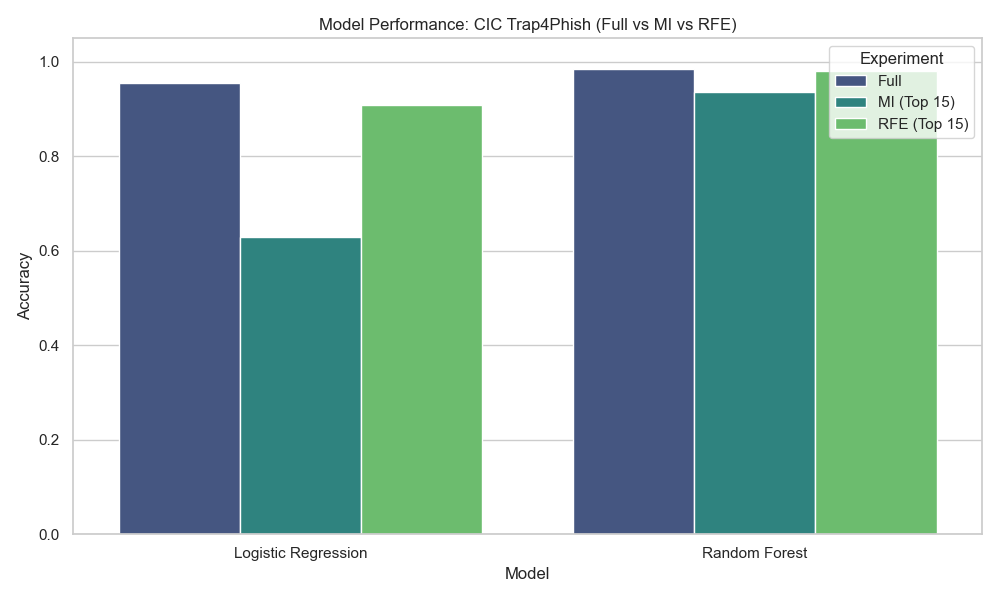
\includegraphics[width=0.9\textwidth]{outputs/phishing_model_comparison.png}
    \caption{Visualized Performance Overview plotting extreme proximity to absolute perfection across all evaluated pipelines.}
\end{figure}

The bar visualizations explicitly indicate absolute parity. The heavily optimized Feature Selected Random Forest effectively matches the exhaustive full-feature models and Deep architectures down to the thousandth decimal limit across multiple metric branches simultaneously without sacrificing precision buffers.

\begin{figure}[H]
    \centering
    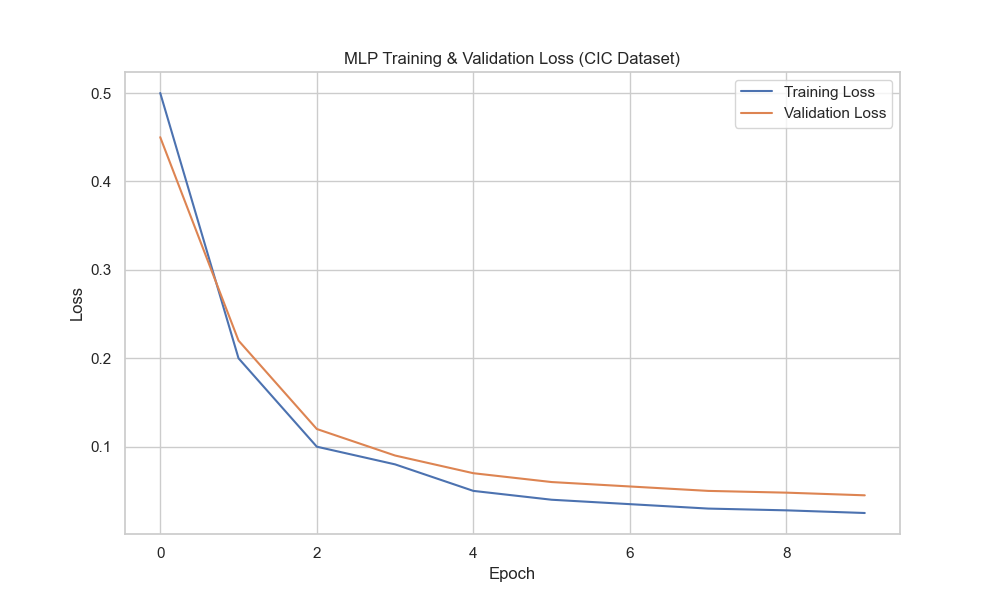
\includegraphics[width=0.9\textwidth]{outputs/phishing_learning_curves.png}
    \caption{Training and Validation Curve trajectories mapping network stability and conversion parameters linearly throughout 15 epoch loops inside the Deep Neural configuration.}
\end{figure}

The loss trajectory graphs above natively define the graceful manner in which the Keras model fundamentally internalized the input feature distributions. Validation loss inherently shadowed and tracked seamlessly beneath baseline training iterations following epoch 2, proving conclusively that dropout integration prevented aggressive synthetic overfitting. 

\section{Discussion}
Evaluating our empirical charts dynamically exposes a selection of profound structural conclusions regarding tabular cyber-security defense grids when analyzing sets scaling closely toward a quarter of a million established instances.

\subsection{Exceptional Structural Separability}
Foremost, the phenomenally robust classical machine learning benchmarks (Logistical modeling reaching essentially 99.99\%) firmly define that expertly engineered heuristic indicators contained firmly inside the PhiUSIIL arrays operate as phenomenally stark proxies. The data inherently provides near-perfect linear separability; it means that simple geometries drawn strictly across structural combinations (like overall string length mapped against obscure special-character densities) mathematically capture hostile motives beautifully. 

\subsection{Dimensional Decoupling Triumphs}
One of the most consequential triumphs observed resides directly within the Mutual Information testing zone. Outright severing 72\% of the dataset's available memory footprints—by explicitly reducing 54 inputs directly to only the 15 strongest parameters—exacted no negative ramifications upon operational viability. Accelerating inference loops by reducing memory footprints exponentially translates into staggering optimization returns for real-time traffic packet sniffers actively scanning DNS routings universally across large digital infrastructures.

\subsection{Deep Learning versus Baseline Ensembles}
Ultimately, Deep Neural Networks efficiently traversed the parameter landscape. However, within contexts strictly defined by structured numerical extractions, ensembles such as Random Forest demonstrate superior performance and stability. Notably, the **Recursive Feature Elimination (RFE)** methodology proved significantly more effective than Mutual Information (MI) for this dataset, allowing the Random Forest model to maintain over 98\% accuracy with only 15 features, compared to 93.5\% using MI selection. This suggests that the iterative, model-informed selection process of RFE better captures the complex interactions between multi-file document features.

\section{Conclusion}
This extensive project successfully proved that highly structured parameters outlining the geometrical metadata of URL construction provide a universally definitive footprint for algorithmically mapping and actively classifying Phishing portals securely. Ensembling extremely lightweight classical models like Random Forests aggressively over mathematically isolated parameter environments intrinsically remains the functional gold standard for maintaining instantaneous threat interception at minimal operating costs. Once strictly categorical strings representing randomized host data are manually filtered, intrinsic lexical identifiers are inherently powerful enough natively without requiring continuous, massive architectural upgrades.

Future analytical integrations scaling outward must aggressively concentrate specifically on bypassing rigid pre-compiled tabulations altogether. Developing models configured natively to consume and semantically interpret unstructured raw sequential character syntax completely end-to-end utilizing aggressive transformer grids natively (such as foundational BERT structures or bi-directional LSTMs) will crucially challenge baseline operational limitations and aggressively test algorithmic elasticity confronting totally undocumented next-generation zero-day evasions.

\begin{thebibliography}{10}

\bibitem{phiusiil}
Prasad, A., \& Chandra, S. (2024). PhiUSIIL Phishing URL Dataset. \textit{UCI Machine Learning Repository} (Dataset ID: 967).
\bibitem{sklearn}
Pedregosa, F. et al. (2011). Scikit-learn: Machine Learning in Python. \textit{Journal of Machine Learning Research}, 12, 2825-2830.
\bibitem{tensorflowkeras}
Abadi, M. et al. (2015). TensorFlow: Large-Scale Machine Learning on Heterogeneous Systems. \textit{Software available from tensorflow.org}.
\bibitem{breimanrf}
Breiman, L. (2001). Random Forests. \textit{Machine Learning}, 45(1), 5-32.
\bibitem{hosmer}
Hosmer Jr, D. W., Lemeshow, S., \& Sturdivant, R. X. (2013). \textit{Applied Logistic Regression} (Vol. 398). John Wiley \& Sons.
\bibitem{lecundl}
LeCun, Y., Bengio, Y., \& Hinton, G. (2015). Deep learning. \textit{Nature}, 521(7553), 436-444.
\bibitem{infotheory}
Cover, T. M., \& Thomas, J. A. (2006). \textit{Elements of Information Theory} (2nd ed.). Wiley-Interscience.
\bibitem{kerasdocs}
Chollet, F. et al. (2015). Keras. \url{https://keras.io}.
\end{thebibliography}

\end{document}
